% Options for packages loaded elsewhere
\PassOptionsToPackage{unicode}{hyperref}
\PassOptionsToPackage{hyphens}{url}
\PassOptionsToPackage{dvipsnames,svgnames*,x11names*}{xcolor}
%
\documentclass[
]{article}
\usepackage{lmodern}
\usepackage{amssymb,amsmath}
\usepackage{ifxetex,ifluatex}
\ifnum 0\ifxetex 1\fi\ifluatex 1\fi=0 % if pdftex
  \usepackage[T1]{fontenc}
  \usepackage[utf8]{inputenc}
  \usepackage{textcomp} % provide euro and other symbols
\else % if luatex or xetex
  \usepackage{unicode-math}
  \defaultfontfeatures{Scale=MatchLowercase}
  \defaultfontfeatures[\rmfamily]{Ligatures=TeX,Scale=1}
\fi
% Use upquote if available, for straight quotes in verbatim environments
\IfFileExists{upquote.sty}{\usepackage{upquote}}{}
\IfFileExists{microtype.sty}{% use microtype if available
  \usepackage[]{microtype}
  \UseMicrotypeSet[protrusion]{basicmath} % disable protrusion for tt fonts
}{}
\makeatletter
\@ifundefined{KOMAClassName}{% if non-KOMA class
  \IfFileExists{parskip.sty}{%
    \usepackage{parskip}
  }{% else
    \setlength{\parindent}{0pt}
    \setlength{\parskip}{6pt plus 2pt minus 1pt}}
}{% if KOMA class
  \KOMAoptions{parskip=half}}
\makeatother
\usepackage{xcolor}
\IfFileExists{xurl.sty}{\usepackage{xurl}}{} % add URL line breaks if available
\IfFileExists{bookmark.sty}{\usepackage{bookmark}}{\usepackage{hyperref}}
\hypersetup{
  pdftitle={Homework 6},
  pdfauthor={Yunting Chiu},
  colorlinks=true,
  linkcolor=red,
  filecolor=Maroon,
  citecolor=Blue,
  urlcolor=blue,
  pdfcreator={LaTeX via pandoc}}
\urlstyle{same} % disable monospaced font for URLs
\usepackage[margin=1in]{geometry}
\usepackage{color}
\usepackage{fancyvrb}
\newcommand{\VerbBar}{|}
\newcommand{\VERB}{\Verb[commandchars=\\\{\}]}
\DefineVerbatimEnvironment{Highlighting}{Verbatim}{commandchars=\\\{\}}
% Add ',fontsize=\small' for more characters per line
\usepackage{framed}
\definecolor{shadecolor}{RGB}{248,248,248}
\newenvironment{Shaded}{\begin{snugshade}}{\end{snugshade}}
\newcommand{\AlertTok}[1]{\textcolor[rgb]{0.94,0.16,0.16}{#1}}
\newcommand{\AnnotationTok}[1]{\textcolor[rgb]{0.56,0.35,0.01}{\textbf{\textit{#1}}}}
\newcommand{\AttributeTok}[1]{\textcolor[rgb]{0.77,0.63,0.00}{#1}}
\newcommand{\BaseNTok}[1]{\textcolor[rgb]{0.00,0.00,0.81}{#1}}
\newcommand{\BuiltInTok}[1]{#1}
\newcommand{\CharTok}[1]{\textcolor[rgb]{0.31,0.60,0.02}{#1}}
\newcommand{\CommentTok}[1]{\textcolor[rgb]{0.56,0.35,0.01}{\textit{#1}}}
\newcommand{\CommentVarTok}[1]{\textcolor[rgb]{0.56,0.35,0.01}{\textbf{\textit{#1}}}}
\newcommand{\ConstantTok}[1]{\textcolor[rgb]{0.00,0.00,0.00}{#1}}
\newcommand{\ControlFlowTok}[1]{\textcolor[rgb]{0.13,0.29,0.53}{\textbf{#1}}}
\newcommand{\DataTypeTok}[1]{\textcolor[rgb]{0.13,0.29,0.53}{#1}}
\newcommand{\DecValTok}[1]{\textcolor[rgb]{0.00,0.00,0.81}{#1}}
\newcommand{\DocumentationTok}[1]{\textcolor[rgb]{0.56,0.35,0.01}{\textbf{\textit{#1}}}}
\newcommand{\ErrorTok}[1]{\textcolor[rgb]{0.64,0.00,0.00}{\textbf{#1}}}
\newcommand{\ExtensionTok}[1]{#1}
\newcommand{\FloatTok}[1]{\textcolor[rgb]{0.00,0.00,0.81}{#1}}
\newcommand{\FunctionTok}[1]{\textcolor[rgb]{0.00,0.00,0.00}{#1}}
\newcommand{\ImportTok}[1]{#1}
\newcommand{\InformationTok}[1]{\textcolor[rgb]{0.56,0.35,0.01}{\textbf{\textit{#1}}}}
\newcommand{\KeywordTok}[1]{\textcolor[rgb]{0.13,0.29,0.53}{\textbf{#1}}}
\newcommand{\NormalTok}[1]{#1}
\newcommand{\OperatorTok}[1]{\textcolor[rgb]{0.81,0.36,0.00}{\textbf{#1}}}
\newcommand{\OtherTok}[1]{\textcolor[rgb]{0.56,0.35,0.01}{#1}}
\newcommand{\PreprocessorTok}[1]{\textcolor[rgb]{0.56,0.35,0.01}{\textit{#1}}}
\newcommand{\RegionMarkerTok}[1]{#1}
\newcommand{\SpecialCharTok}[1]{\textcolor[rgb]{0.00,0.00,0.00}{#1}}
\newcommand{\SpecialStringTok}[1]{\textcolor[rgb]{0.31,0.60,0.02}{#1}}
\newcommand{\StringTok}[1]{\textcolor[rgb]{0.31,0.60,0.02}{#1}}
\newcommand{\VariableTok}[1]{\textcolor[rgb]{0.00,0.00,0.00}{#1}}
\newcommand{\VerbatimStringTok}[1]{\textcolor[rgb]{0.31,0.60,0.02}{#1}}
\newcommand{\WarningTok}[1]{\textcolor[rgb]{0.56,0.35,0.01}{\textbf{\textit{#1}}}}
\usepackage{longtable,booktabs}
% Correct order of tables after \paragraph or \subparagraph
\usepackage{etoolbox}
\makeatletter
\patchcmd\longtable{\par}{\if@noskipsec\mbox{}\fi\par}{}{}
\makeatother
% Allow footnotes in longtable head/foot
\IfFileExists{footnotehyper.sty}{\usepackage{footnotehyper}}{\usepackage{footnote}}
\makesavenoteenv{longtable}
\usepackage{graphicx,grffile}
\makeatletter
\def\maxwidth{\ifdim\Gin@nat@width>\linewidth\linewidth\else\Gin@nat@width\fi}
\def\maxheight{\ifdim\Gin@nat@height>\textheight\textheight\else\Gin@nat@height\fi}
\makeatother
% Scale images if necessary, so that they will not overflow the page
% margins by default, and it is still possible to overwrite the defaults
% using explicit options in \includegraphics[width, height, ...]{}
\setkeys{Gin}{width=\maxwidth,height=\maxheight,keepaspectratio}
% Set default figure placement to htbp
\makeatletter
\def\fps@figure{htbp}
\makeatother
\setlength{\emergencystretch}{3em} % prevent overfull lines
\providecommand{\tightlist}{%
  \setlength{\itemsep}{0pt}\setlength{\parskip}{0pt}}
\setcounter{secnumdepth}{-\maxdimen} % remove section numbering

\title{Homework 6}
\author{Yunting Chiu}
\date{2021-03-23}

\begin{document}
\maketitle

\begin{enumerate}
\def\labelenumi{\arabic{enumi}.}
\tightlist
\item
  (\textbf{6.3}) A student stated: ``Adding predictor variables to a
  regression model can never reduce \(R^2\), so we should include all
  available predictor variables in the model.'' Comment.
\end{enumerate}

\begin{itemize}
\tightlist
\item
  Not really. If the model have a bigger \(R^2\) value, which means the
  fitter is better. However, better fitting does not necessarily imply
  the fitted model is a useful one.
\end{itemize}

\begin{enumerate}
\def\labelenumi{\arabic{enumi}.}
\setcounter{enumi}{1}
\tightlist
\item
  (\textbf{6.4}) Why is it not meaningful to attach a sign to the
  coefficient of multiple correlation R, although we do so for the
  coefficient of simple correlation \(r_{12}\)?
\end{enumerate}

\begin{itemize}
\tightlist
\item
  The range of simple correlation coefficient is -1 to 1. The multiple
  correlation shows how any variable can be predicted by using a set of
  other variables. There will be several independent variables, each of
  which will have a different effect. The multiple correlation
  coefficient will be more complicated than the simple one because the
  range is not limited to -1 to 1.
\end{itemize}

\begin{enumerate}
\def\labelenumi{\arabic{enumi}.}
\setcounter{enumi}{2}
\tightlist
\item
  (\textbf{6.27}) In a small-scale regression study, the following data
  were obtained,
\end{enumerate}

\begin{longtable}[]{@{}lcr@{}}
\toprule
Y & X1 & X2\tabularnewline
\midrule
\endhead
42.0 & 7.0 & 33.0\tabularnewline
33.0 & 4.0 & 41.0\tabularnewline
75.0 & 16.0 & 7.0\tabularnewline
28.0 & 3.0 & 49.0\tabularnewline
91.0 & 21.0 & 5.0\tabularnewline
55.0 & 8.0 & 31.0\tabularnewline
\bottomrule
\end{longtable}

Assume the standard multiple regression model with independent normal
error terms. Compute \textbf{b, e, H,} SSErr, \(R^2\), \(s^2_b\),
\(\hat{Y}\) for \(X1\) = 10, \(X2\) = 30. You can do the computations
using software or by hand, although it would be lengthy to do them by
hand.

\begin{itemize}
\tightlist
\item
  The first column is \texttt{scalar} (1, 1, 1, 1, 1, 1)
\end{itemize}

\begin{Shaded}
\begin{Highlighting}[]
\NormalTok{scalar <-}\StringTok{ }\KeywordTok{c}\NormalTok{(}\DecValTok{1}\NormalTok{, }\DecValTok{1}\NormalTok{, }\DecValTok{1}\NormalTok{, }\DecValTok{1}\NormalTok{, }\DecValTok{1}\NormalTok{, }\DecValTok{1}\NormalTok{)}
\NormalTok{Y <-}\StringTok{  }\KeywordTok{c}\NormalTok{(}\DecValTok{42}\NormalTok{, }\DecValTok{33}\NormalTok{, }\DecValTok{75}\NormalTok{, }\DecValTok{28}\NormalTok{, }\DecValTok{91}\NormalTok{, }\DecValTok{55}\NormalTok{)}
\NormalTok{X1 <-}\StringTok{  }\KeywordTok{c}\NormalTok{(}\DecValTok{7}\NormalTok{, }\DecValTok{4}\NormalTok{, }\DecValTok{16}\NormalTok{, }\DecValTok{3}\NormalTok{, }\DecValTok{21}\NormalTok{, }\DecValTok{8}\NormalTok{)}
\NormalTok{X2 <-}\StringTok{  }\KeywordTok{c}\NormalTok{(}\DecValTok{33}\NormalTok{, }\DecValTok{41}\NormalTok{, }\DecValTok{7}\NormalTok{, }\DecValTok{49}\NormalTok{, }\DecValTok{5}\NormalTok{, }\DecValTok{31}\NormalTok{)}

\CommentTok{# namely X is the matrix}
\NormalTok{X <-}\StringTok{ }\KeywordTok{matrix}\NormalTok{(}\KeywordTok{c}\NormalTok{(scalar, X1, X2), }\DecValTok{6}\NormalTok{, }\DecValTok{3}\NormalTok{, }\DataTypeTok{byrow =} \OtherTok{FALSE}\NormalTok{)}
\NormalTok{X}
\end{Highlighting}
\end{Shaded}

\begin{verbatim}
##      [,1] [,2] [,3]
## [1,]    1    7   33
## [2,]    1    4   41
## [3,]    1   16    7
## [4,]    1    3   49
## [5,]    1   21    5
## [6,]    1    8   31
\end{verbatim}

\hypertarget{b-slope}{%
\subsection{b: slope}\label{b-slope}}

\[
\boldsymbol{\hat{\beta}} = \boldsymbol{(X^TX)}^{-1}\boldsymbol{(X^TY)}
\]

\begin{Shaded}
\begin{Highlighting}[]
\KeywordTok{library}\NormalTok{(matlib)}
\NormalTok{b =}\StringTok{ }\KeywordTok{inv}\NormalTok{(}\KeywordTok{t}\NormalTok{(X) }\OperatorTok\StringTok{ }\NormalTok{X) }\OperatorTok\StringTok{ }\KeywordTok{t}\NormalTok{(X) }\OperatorTok\StringTok{ }\NormalTok{Y}
\NormalTok{b}
\end{Highlighting}
\end{Shaded}

\begin{verbatim}
##            [,1]
## [1,] 33.9321020
## [2,]  2.7847707
## [3,] -0.2643979
\end{verbatim}

\hypertarget{h-hat}{%
\subsection{H: Hat}\label{h-hat}}

\begin{itemize}
\tightlist
\item
  H is called the hat-matrix (because it transforms \(y\) to
  \(\hat{y}\)) \[
  H = X\boldsymbol{(X^TX)}^{-1}\boldsymbol{X^T}
  \]
\end{itemize}

\begin{Shaded}
\begin{Highlighting}[]
\NormalTok{H =}\StringTok{ }\NormalTok{X }\OperatorTok\StringTok{ }\KeywordTok{inv}\NormalTok{(}\KeywordTok{t}\NormalTok{(X) }\OperatorTok\StringTok{ }\NormalTok{X) }\OperatorTok\StringTok{ }\KeywordTok{t}\NormalTok{(X)}
\NormalTok{H}
\end{Highlighting}
\end{Shaded}

\begin{verbatim}
##             [,1]        [,2]        [,3]       [,4]        [,5]       [,6]
## [1,]  0.23143639  0.25168006  0.21178834  0.1488734 -0.05475455 0.21099418
## [2,]  0.25168006  0.31240977  0.09437951  0.2662835 -0.14787196 0.22314063
## [3,]  0.21178834  0.09437951  0.70442097 -0.3191731  0.10446756 0.20412257
## [4,]  0.14887339  0.26628346 -0.31917314  0.6142637  0.14143589 0.14834214
## [5,] -0.05475455 -0.14787196  0.10446756  0.1414359  0.94040059 0.01632796
## [6,]  0.21099418  0.22314063  0.20412257  0.1483421  0.01632796 0.19708945
\end{verbatim}

\hypertarget{e-resuduals}{%
\subsection{e: resuduals}\label{e-resuduals}}

\[
e = Y -\hat{Y} = Y - H * Y
\]

\begin{Shaded}
\begin{Highlighting}[]
\NormalTok{e <-}\StringTok{ }\NormalTok{Y }\OperatorTok{-}\StringTok{ }\NormalTok{H }\OperatorTok\StringTok{ }\NormalTok{Y}
\NormalTok{e}
\end{Highlighting}
\end{Shaded}

\begin{verbatim}
##             [,1]
## [1,] -2.70036663
## [2,] -1.23087135
## [3,] -1.63764825
## [4,] -1.33091751
## [5,] -0.09029763
## [6,]  6.98606687
\end{verbatim}

\hypertarget{sserr}{%
\subsection{SSErr}\label{sserr}}

\[
SSE = e^T * e
\]

\begin{itemize}
\tightlist
\item
  \textbf{SSErr} is error sum of squares.
\end{itemize}

\begin{Shaded}
\begin{Highlighting}[]
\NormalTok{SSE <-}\StringTok{ }\KeywordTok{t}\NormalTok{(e) }\OperatorTok\StringTok{ }\NormalTok{e}
\NormalTok{SSE}
\end{Highlighting}
\end{Shaded}

\begin{verbatim}
##          [,1]
## [1,] 62.07354
\end{verbatim}

\begin{Shaded}
\begin{Highlighting}[]
\CommentTok{# SSErr <- sum(e^2)}
\CommentTok{# SSErr}
\end{Highlighting}
\end{Shaded}

\hypertarget{r2}{%
\subsection{\texorpdfstring{\textbf{\(R^2\)}}{R\^{}2}}\label{r2}}

\[
R^2 = \frac{SSRegression}{SSTotal} = 1 - \frac{SSError}{SSTotal}
\]

\begin{Shaded}
\begin{Highlighting}[]
\NormalTok{SST <-}\StringTok{ }\KeywordTok{sum}\NormalTok{((Y }\OperatorTok{-}\StringTok{ }\KeywordTok{mean}\NormalTok{(Y))}\OperatorTok{^}\DecValTok{2}\NormalTok{) }\CommentTok{# total sum of squares}
\NormalTok{SST}
\end{Highlighting}
\end{Shaded}

\begin{verbatim}
## [1] 3072
\end{verbatim}

\begin{Shaded}
\begin{Highlighting}[]
\NormalTok{R2 <-}\StringTok{ }\DecValTok{1} \OperatorTok{-}\StringTok{ }\NormalTok{SSE}\OperatorTok{/}\NormalTok{SST }\CommentTok{# R^2}
\NormalTok{R2}
\end{Highlighting}
\end{Shaded}

\begin{verbatim}
##           [,1]
## [1,] 0.9797938
\end{verbatim}

\hypertarget{s2_b}{%
\subsection{\texorpdfstring{\textbf{\(s^2_b\)}}{s\^{}2\_b}}\label{s2_b}}

\[
MSE = \frac{SSE}{n-2}
\]

\begin{Shaded}
\begin{Highlighting}[]
\NormalTok{MSE <-}\StringTok{ }\NormalTok{SSE}\OperatorTok{/}\StringTok{ }\NormalTok{(}\DecValTok{6-2}\NormalTok{)}
\NormalTok{MSE}
\end{Highlighting}
\end{Shaded}

\begin{verbatim}
##          [,1]
## [1,] 15.51839
\end{verbatim}

\[
S^2\{b\} = MSE(X^T * X)^{-1}
\]

\begin{Shaded}
\begin{Highlighting}[]
\NormalTok{s2b <-}\StringTok{ }\NormalTok{MSE[}\DecValTok{1}\NormalTok{,}\DecValTok{1}\NormalTok{] }\OperatorTok{*}\StringTok{ }\KeywordTok{inv}\NormalTok{(}\KeywordTok{t}\NormalTok{(X) }\OperatorTok\StringTok{ }\NormalTok{X)}
\NormalTok{s2b}
\end{Highlighting}
\end{Shaded}

\begin{verbatim}
##           [,1]        [,2]        [,3]
## [1,] 536.60338 -25.6191888 -10.1962033
## [2,] -25.61919   1.2462499   0.4830506
## [3,] -10.19620   0.4830506   0.1968509
\end{verbatim}

\hypertarget{eyx1-10-x2-30}{%
\subsection{E\{Y\textbar X1 = 10, X2 = 30\}}\label{eyx1-10-x2-30}}

\begin{itemize}
\tightlist
\item
  The equation below is an unbiased estimator of estimated of Y\_n. \[
  \hat{Y}_h = X_h^T * b
  \]
\end{itemize}

\begin{Shaded}
\begin{Highlighting}[]
\NormalTok{Xone <-}\StringTok{ }\KeywordTok{c}\NormalTok{(}\DecValTok{1}\NormalTok{, }\DecValTok{10}\NormalTok{, }\DecValTok{30}\NormalTok{)}
\NormalTok{yhat <-}\StringTok{ }\KeywordTok{t}\NormalTok{(Xone) }\OperatorTok\StringTok{ }\NormalTok{b}
\NormalTok{yhat}
\end{Highlighting}
\end{Shaded}

\begin{verbatim}
##          [,1]
## [1,] 53.84787
\end{verbatim}

\begin{itemize}
\tightlist
\item
  Reference:

  \begin{itemize}
  \tightlist
  \item
    \url{https://stats.stackexchange.com/questions/352130/converting-the-beta-coefficient-from-matrix-to-scalar-notation-in-ols-regression}
  \item
    \url{https://www.stat.cmu.edu/~cshalizi/mreg/15/lectures/13/lecture-13.pdf}
  \item
    \url{http://fs2.american.edu/baron/www/Handouts/review\%20-\%20regression.pdf}
  \end{itemize}
\end{itemize}

\begin{enumerate}
\def\labelenumi{\arabic{enumi}.}
\setcounter{enumi}{3}
\tightlist
\item
  (Computer project, \textbf{\#6.5---\#6.8}) Dataset ``Brand
  preference'' is available on our Blackboard, on
  \url{http://statweb.lsu.edu/EXSTWeb/StatLab/DataSets/NKNWData/CH06PR05.txt},
  and here:
\end{enumerate}

\begin{Shaded}
\begin{Highlighting}[]
\NormalTok{brand <-}\StringTok{ }\KeywordTok{read.table}\NormalTok{(}\StringTok{"./data/CH06PR05.txt"}\NormalTok{)}
\NormalTok{brand }\OperatorTok
\StringTok{  }\KeywordTok{rename}\NormalTok{(}\DataTypeTok{brand =} \StringTok{"V1"}\NormalTok{, }\DataTypeTok{moisture =} \StringTok{"V2"}\NormalTok{, }\DataTypeTok{sweetness =} \StringTok{"V3"}\NormalTok{) ->}\StringTok{ }\NormalTok{brand}
\NormalTok{brand}
\end{Highlighting}
\end{Shaded}

\begin{verbatim}
##    brand moisture sweetness
## 1     64        4         2
## 2     73        4         4
## 3     61        4         2
## 4     76        4         4
## 5     72        6         2
## 6     80        6         4
## 7     71        6         2
## 8     83        6         4
## 9     83        8         2
## 10    89        8         4
## 11    86        8         2
## 12    93        8         4
## 13    88       10         2
## 14    95       10         4
## 15    94       10         2
## 16   100       10         4
\end{verbatim}

\begin{Shaded}
\begin{Highlighting}[]
\CommentTok{# Y, X1, X2}
\end{Highlighting}
\end{Shaded}

It was collected to study the relation between degree of brand liking (Y
) and moisture content (X1) and sweetness (X2) of the product. (a) Fit a
regression model to these data and state the estimated regression
function. Interpret b1. \[
\hat{Y} = 37.6500 + 4.4250X1 + 4.3750X2
\] - The slope \(b_1\) is 4.425, meaning that the mean response
\texttt{degree\ of\ brand\ liking} is increase by 4.425 with 1 unit
increase of \texttt{moisture} when \texttt{sweetness} is held constant.

\begin{Shaded}
\begin{Highlighting}[]
\NormalTok{reg <-}\StringTok{ }\KeywordTok{lm}\NormalTok{(brand }\OperatorTok{~}\StringTok{ }\NormalTok{moisture }\OperatorTok{+}\StringTok{ }\NormalTok{sweetness, }\DataTypeTok{data =}\NormalTok{ brand)}
\KeywordTok{summary}\NormalTok{(reg)}
\end{Highlighting}
\end{Shaded}

\begin{verbatim}
## 
## Call:
## lm(formula = brand ~ moisture + sweetness, data = brand)
## 
## Residuals:
##    Min     1Q Median     3Q    Max 
## -4.400 -1.762  0.025  1.587  4.200 
## 
## Coefficients:
##             Estimate Std. Error t value Pr(>|t|)    
## (Intercept)  37.6500     2.9961  12.566 1.20e-08 ***
## moisture      4.4250     0.3011  14.695 1.78e-09 ***
## sweetness     4.3750     0.6733   6.498 2.01e-05 ***
## ---
## Signif. codes:  0 '***' 0.001 '**' 0.01 '*' 0.05 '.' 0.1 ' ' 1
## 
## Residual standard error: 2.693 on 13 degrees of freedom
## Multiple R-squared:  0.9521, Adjusted R-squared:  0.9447 
## F-statistic: 129.1 on 2 and 13 DF,  p-value: 2.658e-09
\end{verbatim}

\begin{enumerate}
\def\labelenumi{(\alph{enumi})}
\setcounter{enumi}{1}
\tightlist
\item
  Obtain residual plots. What information do they provide? Plot
  residuals against fitted values, against each predictor, and against
  the product of predictors.
\end{enumerate}

\begin{itemize}
\tightlist
\item
  We need to make residual plots to see if the data points meet the
  linear assumptions or not.
\item
  Residuals vs Fitted plot: a strong pattern indicates non-linearity in
  the data
\item
  Normal QQ plot: Some outliers can be found in the right upper area. It
  is necessary to conduct further testing.
\item
  Scale-Location: The residuals seem symmetric and the red line is
  approximately horizontal. However, the average magnitude of the
  standardized residuals is not changing much as a function of the
  fitted values.
\item
  Residual vs Leverage: There are some potential outliers can be found
  in the right side. Reference:
  \url{https://boostedml.com/2019/03/linear-regression-plots-scale-location-plot.html}
\end{itemize}

\begin{Shaded}
\begin{Highlighting}[]
\KeywordTok{par}\NormalTok{(}\DataTypeTok{mfrow =} \KeywordTok{c}\NormalTok{(}\DecValTok{2}\NormalTok{, }\DecValTok{2}\NormalTok{))}
\KeywordTok{plot}\NormalTok{(reg)}
\end{Highlighting}
\end{Shaded}

\includegraphics{YuntingChiu_hw6_files/figure-latex/unnamed-chunk-12-1.pdf}

\begin{enumerate}
\def\labelenumi{(\alph{enumi})}
\setcounter{enumi}{2}
\tightlist
\item
  Test homoscedasticity.
\end{enumerate}

\begin{itemize}
\tightlist
\item
  With a high p-value 0.42877, there is no evidence of non-constant
  variance.
\end{itemize}

\begin{Shaded}
\begin{Highlighting}[]
\KeywordTok{library}\NormalTok{(car)}
\end{Highlighting}
\end{Shaded}

\begin{verbatim}
## Loading required package: carData
\end{verbatim}

\begin{verbatim}
## 
## Attaching package: 'car'
\end{verbatim}

\begin{verbatim}
## The following object is masked from 'package:dplyr':
## 
##     recode
\end{verbatim}

\begin{verbatim}
## The following object is masked from 'package:purrr':
## 
##     some
\end{verbatim}

\begin{Shaded}
\begin{Highlighting}[]
\KeywordTok{ncvTest}\NormalTok{(reg)}
\end{Highlighting}
\end{Shaded}

\begin{verbatim}
## Non-constant Variance Score Test 
## Variance formula: ~ fitted.values 
## Chisquare = 0.6261627, Df = 1, p = 0.42877
\end{verbatim}

\begin{enumerate}
\def\labelenumi{(\alph{enumi})}
\setcounter{enumi}{3}
\tightlist
\item
  Conduct a formal lack of fit test.
\end{enumerate}

\begin{itemize}
\tightlist
\item
  We conclude that the p-value is 0.3843, we fail to reject the H0,
  meaning that there is no evidence of lack of fit. Thus, there should
  be no significant difference in error between estimates from the
  reduced (\texttt{reg}) model and the full model.
\item
  Reference:
  \url{https://stats.stackexchange.com/questions/339331/difference-between-full-model-and-reduced-model-in-one-way-anova}
  \[
  Full Model: Y_{ij} = \mu_j + e_{ij}
  \] \[
  Reduced Model: Y_{ij} = \mu + e_{ij}
  \]
\end{itemize}

\begin{Shaded}
\begin{Highlighting}[]
\NormalTok{full <-}\StringTok{ }\KeywordTok{lm}\NormalTok{(brand }\OperatorTok{~}\StringTok{ }\KeywordTok{as.factor}\NormalTok{(moisture) }\OperatorTok{+}\StringTok{ }\KeywordTok{as.factor}\NormalTok{(sweetness), }\DataTypeTok{data =}\NormalTok{ brand)}
\KeywordTok{anova}\NormalTok{(reg, full)}
\end{Highlighting}
\end{Shaded}

\begin{verbatim}
## Analysis of Variance Table
## 
## Model 1: brand ~ moisture + sweetness
## Model 2: brand ~ as.factor(moisture) + as.factor(sweetness)
##   Res.Df   RSS Df Sum of Sq      F Pr(>F)
## 1     13 94.30                           
## 2     11 79.25  2     15.05 1.0445 0.3843
\end{verbatim}

\begin{enumerate}
\def\labelenumi{(\alph{enumi})}
\setcounter{enumi}{4}
\tightlist
\item
  Test whether the proposed linear regression model is significant. What
  do the results of the ANOVA F-test imply about the slopes?
\end{enumerate}

\begin{itemize}
\tightlist
\item
  Let we set H0: \(\beta1 = \beta2 = 0\) vs Ha: \$\beta1 \neq0 or \beta2
  \neq0 \$ at least.
\item
  We found both p-values (\(\beta1\) and \(\beta2\)) are smaller than
  significant level, implying that we are in favor of Ha. Reference:
  \url{https://www.researchgate.net/post/Is_the_null_and_alternative_hypothesis_for_this_multiple_linear_regression_analysis_correct}
\end{itemize}

\begin{Shaded}
\begin{Highlighting}[]
\KeywordTok{anova}\NormalTok{(reg)}
\end{Highlighting}
\end{Shaded}

\begin{verbatim}
## Analysis of Variance Table
## 
## Response: brand
##           Df  Sum Sq Mean Sq F value    Pr(>F)    
## moisture   1 1566.45 1566.45 215.947 1.778e-09 ***
## sweetness  1  306.25  306.25  42.219 2.011e-05 ***
## Residuals 13   94.30    7.25                      
## ---
## Signif. codes:  0 '***' 0.001 '**' 0.01 '*' 0.05 '.' 0.1 ' ' 1
\end{verbatim}

\begin{Shaded}
\begin{Highlighting}[]
\KeywordTok{summary}\NormalTok{(reg)}
\end{Highlighting}
\end{Shaded}

\begin{verbatim}
## 
## Call:
## lm(formula = brand ~ moisture + sweetness, data = brand)
## 
## Residuals:
##    Min     1Q Median     3Q    Max 
## -4.400 -1.762  0.025  1.587  4.200 
## 
## Coefficients:
##             Estimate Std. Error t value Pr(>|t|)    
## (Intercept)  37.6500     2.9961  12.566 1.20e-08 ***
## moisture      4.4250     0.3011  14.695 1.78e-09 ***
## sweetness     4.3750     0.6733   6.498 2.01e-05 ***
## ---
## Signif. codes:  0 '***' 0.001 '**' 0.01 '*' 0.05 '.' 0.1 ' ' 1
## 
## Residual standard error: 2.693 on 13 degrees of freedom
## Multiple R-squared:  0.9521, Adjusted R-squared:  0.9447 
## F-statistic: 129.1 on 2 and 13 DF,  p-value: 2.658e-09
\end{verbatim}

\begin{enumerate}
\def\labelenumi{(\alph{enumi})}
\setcounter{enumi}{5}
\tightlist
\item
  Estimate both slopes simultaneously using the Bonferroni procedure
  with at least a 99 percent confidence level.
\end{enumerate}

\begin{itemize}
\tightlist
\item
  The Bonferroni test is a statistical test used to reduce the instance
  of a false positive (typr 1 error)
\item
  To preform the Bonferroni correction, we need to divide the \(\alpha\)
  level by the number of tests that being executed.
\item
  We need to test 2 slopes, and the significance level is 0.01. So,
  0.01/2 = 0.005. Throughout the Bonferroni procedure, the adjusted
  \(alpha\) level is 0.005 with two slopes.
\item
  Reference: \url{https://toptipbio.com/bonferroni-correction-method/}
\end{itemize}

\begin{Shaded}
\begin{Highlighting}[]
\KeywordTok{confint}\NormalTok{(reg, }\DataTypeTok{level =}\NormalTok{ (}\DecValTok{1}\FloatTok{-0.005}\NormalTok{))}
\end{Highlighting}
\end{Shaded}

\begin{verbatim}
##                0.25 %   99.75 %
## (Intercept) 27.545738 47.754262
## moisture     3.409483  5.440517
## sweetness    2.104236  6.645764
\end{verbatim}

\begin{enumerate}
\def\labelenumi{(\alph{enumi})}
\setcounter{enumi}{6}
\tightlist
\item
  Report R2 and adjusted R2. How are they interpreted here?
\end{enumerate}

\begin{itemize}
\tightlist
\item
  It means that 95 \% of the variation in the \texttt{brand} is
  explained by the \texttt{moisture} and \texttt{sweetness} independent
  variables.
\end{itemize}

\begin{Shaded}
\begin{Highlighting}[]
\KeywordTok{summary}\NormalTok{(reg)}\OperatorTok{$}\NormalTok{r.square}
\end{Highlighting}
\end{Shaded}

\begin{verbatim}
## [1] 0.952059
\end{verbatim}

\begin{itemize}
\tightlist
\item
  It means that 94 \% of the variation in the \texttt{brand} is
  explained by model addition that are significant of \texttt{moisture}
  and \texttt{sweetness}.
\end{itemize}

\begin{Shaded}
\begin{Highlighting}[]
\KeywordTok{summary}\NormalTok{(reg)}\OperatorTok{$}\NormalTok{adj.r.square}
\end{Highlighting}
\end{Shaded}

\begin{verbatim}
## [1] 0.9446834
\end{verbatim}

\begin{itemize}
\tightlist
\item
  Reference:
  \url{https://discuss.analyticsvidhya.com/t/difference-between-r-square-and-adjusted-r-square/264/2}
\end{itemize}

\begin{enumerate}
\def\labelenumi{(\alph{enumi})}
\setcounter{enumi}{7}
\tightlist
\item
  Calculate the squared correlation coefficient between \(Yi\) and
  \(\hat{Y}\). Compare with part (g).
\end{enumerate}

\begin{itemize}
\tightlist
\item
  The squared correlation coefficient between \(Yi\) and \(\hat{Y}\) is
  \(R^2\), which is 0.952059.
\end{itemize}

\begin{enumerate}
\def\labelenumi{(\roman{enumi})}
\tightlist
\item
  Obtain a 99\% confidence interval for E(Y) when X1 = 5 and X2 = 4.
  Interpret it.
\end{enumerate}

\begin{itemize}
\tightlist
\item
  We have 99 \% confidence to conclude that the \textbf{mean} of
  \texttt{degree\ of\ brand\ liking} is between 73.88111 to 80.66889
  when the \texttt{moisture\ content} is 5 and the
  \texttt{sweetness\ of\ the\ product} is 4.
\end{itemize}

\begin{Shaded}
\begin{Highlighting}[]
\KeywordTok{predict}\NormalTok{(reg, }\KeywordTok{tibble}\NormalTok{(}\DataTypeTok{moisture =} \DecValTok{5}\NormalTok{, }\DataTypeTok{sweetness =} \DecValTok{4}\NormalTok{), }\DataTypeTok{interval =} \StringTok{"confidence"}\NormalTok{, }\DataTypeTok{level =} \FloatTok{0.99}\NormalTok{)}
\end{Highlighting}
\end{Shaded}

\begin{verbatim}
##      fit      lwr      upr
## 1 77.275 73.88111 80.66889
\end{verbatim}

\begin{enumerate}
\def\labelenumi{(\alph{enumi})}
\setcounter{enumi}{9}
\tightlist
\item
  Obtain a 99\% prediction interval for a new observation Y when X1 = 5
  and X2 = 4. Interpret it.
\end{enumerate}

\begin{itemize}
\tightlist
\item
  We have 99 \% confidence to conclude that \textbf{a next new
  observation } of \texttt{degree\ of\ brand\ liking} is between
  73.88111 to 80.66889 when the \texttt{moisture\ content} is 5 and the
  \texttt{sweetness\ of\ the\ product} is 4.
\end{itemize}

\begin{Shaded}
\begin{Highlighting}[]
\KeywordTok{predict}\NormalTok{(reg, }\KeywordTok{tibble}\NormalTok{(}\DataTypeTok{moisture =} \DecValTok{5}\NormalTok{, }\DataTypeTok{sweetness =} \DecValTok{4}\NormalTok{), }\DataTypeTok{interval =} \StringTok{"prediction"}\NormalTok{, }\DataTypeTok{level =} \FloatTok{0.99}\NormalTok{)}
\end{Highlighting}
\end{Shaded}

\begin{verbatim}
##      fit      lwr      upr
## 1 77.275 68.48077 86.06923
\end{verbatim}

\begin{enumerate}
\def\labelenumi{\arabic{enumi}.}
\setcounter{enumi}{4}
\tightlist
\item
  (\textbf{\# 6.26, Stat-615 only}) Show that the squared sample
  correlation coefficient between \(Y\) and \(\hat Y\) equals \(R^2\).
\end{enumerate}

Remark. Now you can check if you did \#3h correctly.\\
Hints. First, show that the sample averages of Yi and Ybi are the same.
Then, write the sample correlation coefficient between \(Y\) and
\(\hat Y\) as \[
 r_{Y\widehat{Y}} = \frac{\sum
 (Y_i-\overline{Y})(\widehat{Y}_i-\overline{Y})}{\sqrt{\sum
 (Y_i-\overline{Y})^2\sum(\widehat{Y}_i-\overline{Y})^2}}
 = \frac{\sum
 (\widehat{Y}_i-\overline{Y}+Y_i-\widehat{Y}_i)(\widehat{Y}_i-\overline{Y})}{\sqrt{\sum
 (Y_i-\overline{Y})^2\sum(\widehat{Y}_i-\overline{Y})^2}}
 \] and use known properties of residuals \(\sum e_i=0\),
\(\sum X_{ij} e_i=0\), \(\sum \widehat{Y}_i e_i=0\). \}\}

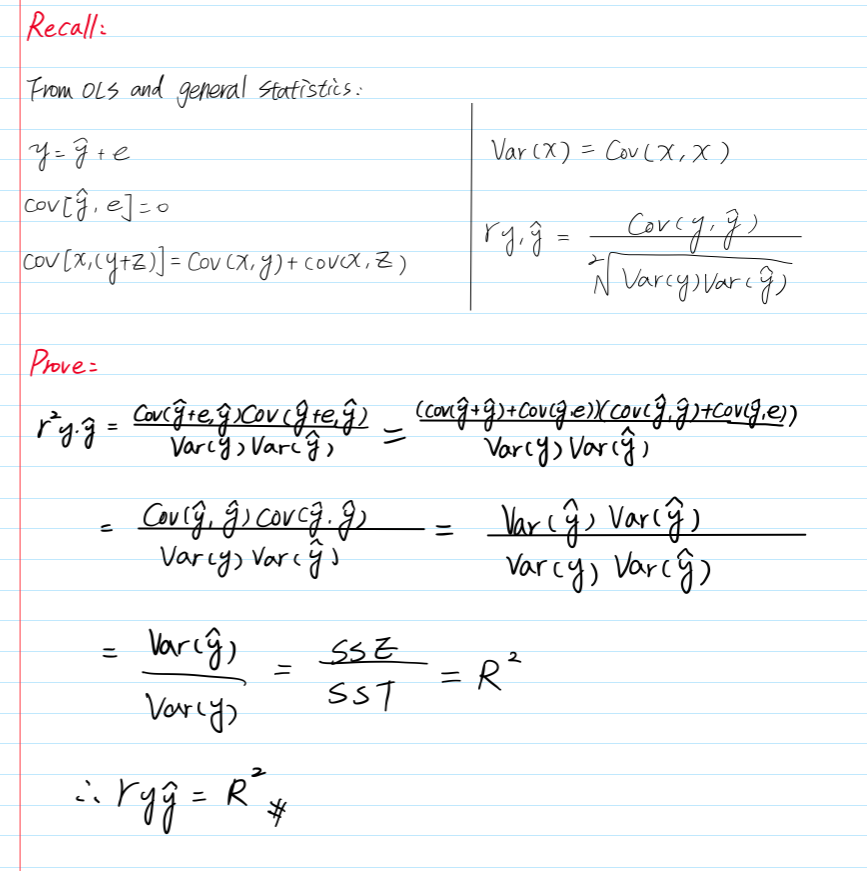
\includegraphics{q6/6.png}

\begin{itemize}
\tightlist
\item
  Reference:
  \url{https://stats.stackexchange.com/questions/187734/relationship-between-r2-and-correlation-coefficient}
\end{itemize}

\end{document}
